\documentclass{gmto}
% Extra LaTeX packages
\usepackage{caption}
\usepackage{subcaption}
% Useful packages
\usepackage{amsmath, amssymb}
\usepackage{siunitx}
\usepackage{biblatex}
% \setlength {\marginparwidth }{2cm}
\usepackage{todonotes}
%\usepackage[colorlinks=true, allcolors=blue]{hyperref}
\newtheorem{remark}{Remark}

\DocID{GMT-DOC-05989}
\DocVersion{1.0}
\DocStatus{Draft}

\addbibresource{gmt.bib}
% \addbibresource{./gmto.bib}

\title{LTAO End-to-End Simulation Model}
%\subtitle{}
\author{R.~Romano and R.~Conan}
\date{December 7, 2023}%\today

\begin{document}

\maketitle

\clearpage

\section*{Signatures}
\vspace{1cm}
\subsection*{Author}
\vspace{1.5cm}
%\tabulinesep=1em
\begin{tabu} to \linewidth {X[3,l]X[1,l]}
  \rule{\linewidth}{.1pt} & \rule{\linewidth}{.1pt} \\
  Name, title & Date
\end{tabu}
\vspace{1.5cm}
\subsection*{Approvers}
\vspace{1.5cm}
%\tabulinesep=1em
\begin{tabu} to \linewidth {X[3,l]X[1,l]}
  \rule{\linewidth}{.1pt} & \rule{\linewidth}{.1pt} \\
  Name, title & Date \\[1cm]
  \rule{\linewidth}{.1pt} & \rule{\linewidth}{.1pt} \\
  Name, title & Date
\end{tabu}

\clearpage

\section*{Revision Log}

\begin{revisions}
  1.0 & \today & All & None & Initial version & Author \\  
\end{revisions}

\clearpage

\tableofcontents
\listoffigures
\listoftables

\clearpage

\section{Purpose}
\label{sec:purpose}

This document describes the end-to-end model representing the Laser Tomography Adaptive Optics (LTAO) observing mode. The current version combines the LTAO wavefront control architecture and a state-space model reproducing the telescope dynamics. Though that state-space model considers a flexible face sheet representation of the ASM, at the moment, we restrict the commands to segment tip-tilt and piston. The motivation behind the LTAO model described in this effort that differs from other efforts is twofold. First, we aim to provide a first-order approximation of the laser tomographic wavefront sensor behavior, particularly regarding the limitation on measuring global tip-tilt. The second is integrating wavefront control and the loops using M1 and M2 edge sensors with other subsystem loops.


\section{Introduction}
\label{sec:introduction}

Figure~\ref{fig:ltaoIM} illustrates the LTAO integrated model for end-to-end simulations. One can split the model into two parts. The first is an inner subsystem comprising a state-space model representing the telescope dynamics and low-level control loops. The second partition has the higher-level controllers relying on optical sensors. 
%
\begin{figure}[!hbt]
    \centering
    \includegraphics[width=\textwidth]{../ltao_e2e-main.pdf}
    \caption{LTAO end-to-end simulation model.}
    \label{fig:ltaoIM}
\end{figure}
%
We consider low-level controllers those interfacing directly with the structural model; that is, their outputs are forces (and torques), which are inputs of the GMT structural model.


There are four low-level control loops in the current version: the mount axes (driving azimuth, elevation, and GIR drive torques), the M1 outer force loop (providing the support actuator forces), the M2 positioner, and the ASM control system. %
%
Though the M2 edge sensor (ES) control loop is not considered low-level according to the previous definition (its output is a set of offset commands handled as reference signals by the ASM controller), it is part of the M2 subsystem. Therefore, we opt to represent it within the dashed box illustrating the inner partition of the simulation model.

The mount axes control model follows ODC's design (refer to \cite{ODC_end2end_2021} for a detailed description). Each axis is controlled independently using a PID compensator and notch filters to cope with structural resonant modes. A feedforward strategy is also envisioned to relieve the feedback compensator during critical acceleration/deceleration phases. The mount control system tuning assumes a structural damping of 2\%. %
%
The M1 control model implements the loop responsible for compensating for the forces acting over the mirror (measured by the hardpoint load cells) through support forces exerted by the array of pneumatic actuators. %
The document \cite{GMT.DOC.05153} thoroughly describes the M1 control system in the context of the GMT integrated model. %

%\section{}

A modal control approach has been considered to improve the computational efficiency of end-to-end simulations based on the flexible face-sheet ASM design. In that approach, we apply input and output orthonormal transformations based on Karhunen-Loève (KL) modal matrix $V_\text{KL}^{(i)}$, which is computed according to the $n_a=675$ coordinates of the nodes of a particular ASM segment. %
%
For each segment $i \in \{1,\ldots,7\}$, the orthonormal matrix $V_\text{KL}^{(i)} \in \mathbb{R}^{n_a \times n_m}$ performs the transformation from a modal basis (modal forces/modal coefficients) in the ASM KL space to a zonal basis in the ASM actuator space (actuator forces/node displacements). The transpose of  $V_\text{KL}^{(i)}$ performs the dual transformation from a zonal basis to a modal basis. %
%
% $V_\text{KL}^{(i)T}$ performs the basis transformation
%
% for each segment $i \in \{1,\ldots,7\}$ composing the ASMS, $V_\text{KL}^{(i)} \in \mathbb{R}^{n_a \times n_m}$ transforms an $n_m$--dimensional vector of modal forces into an $n_a$--dimensional vector of ASM actuator forces. Analogously, $V_\text{KL}^{(i)T}$ projects the axial node displacements onto the KL mode shapes, leading to $n_m$ modal displacement coefficients. 
Thus, in the modal approach, modal coefficients (linear combinations of the node displacements) are fed back to the ASM inner loop controller, which outputs modal forces as control signals. The model version described in this tech note focuses on the first three KL mode shapes: piston, tip, and tilt. Therefore, $n_m=3$ and the matrix $V_\text{012}$ represented in Figure~\ref*{fig:ltaoIM} reads as
\[
V_\text{012} = \begin{bmatrix}
    V_\text{KL}^{(1)} & & \bigcirc \\
    & \ddots & \\
    \bigcirc & & V_\text{KL}^{(7)}
\end{bmatrix}.
\]

The air trapped in the thin gap between the ASM face sheet (FS) and the reference body (RB) is the source of fluid dynamic forces, which load the mirror and the reference body. Those forces are not negligible and can highly characterize the ASM system's performance and stability~\cite{ADP_PhasingRep2021}. %The fluid dynamic forces are nonlinear functions of the gap, the spatial/modal deformation amplitude, and shape of the mirror, and the deformation velocity/frequency. Assuming a frequency range of interest of a few hundredths of Hz, the fluid dynamic forces can be simplified to linear fluid dynamic damping.
%
As shown in Figure~\ref*{fig:ltaoIM}, though the flexible face sheet ASM structural models have considered a wide frequency range (up to \SI{2.1}{kHz}), in this document, we assume a linear fluid dynamic damping representation, with $k_\text{fd}=\SI{9.1}{Ns/m}$.

%
The M2 control system model is approached in previous documents~\cite{GMT.DOC.05553, GMT.DOC.05941}. However, to make this note self-contained, we reproduce the description of the M2 control model in Appendix~\ref{sec:m2_control}.



\section{LTAO Wavefront Control Model}

Figure~\ref{fig:ltao_wfsc_detailed} provides an alternative representation of the LTAO end-to-end simulation model. The block diagram shows the controllers composing the wavefront control architecture in more detail. It also illustrates the interfaces between the high- and the low-level control loops (black dashed line block of Figure~\ref{fig:ltaoIM}).
%
\begin{figure}[!ht]
    \centering
    \includegraphics[width=\textwidth]{../ltao_e2e-detailed_wfsc.pdf}
    \caption[LTAO wavefront control model]{LTAO wavefront control system and its interfaces with the low-level control loops.}
    \label{fig:ltao_wfsc_detailed}
\end{figure}
%

\subsection{Wavefront sensor models}

The linear approximations represent the Laser Tomographic Wavefront Sensor (LTWS)  and the On-Instrument Wavefront Sensor (OIWFS). Let $y_\text{m1} \in \mathbb{R}^{42}$ and $y_\text{m2} \in \mathbb{R}^{42}$ vectors containing the M1 and M2 rigid-body motions, respectively. %vertexes
The GMT linear optical model (LOM) provides the matrices $L_\text{stt} \in \mathbb{R}^{14 \times 84}$, $L_\text{sp} \in \mathbb{R}^{7 \times 84}$, and $L_\text{gtt} \in \mathbb{R}^{2 \times 84}$ such that
\begin{align}
    \begin{bmatrix}
        y_\text{stt} \\ y_\text{sp} \\ y_\text{gtt}
    \end{bmatrix} =
    \begin{bmatrix} 
    L_\text{stt} \\ L_\text{sp} \\ L_\text{gtt}
\end{bmatrix}
    \begin{bmatrix}
    y_\text{m1} \\ y_\text{m2}
    \end{bmatrix}, \label{eq:lom}
\end{align}
where $y_\text{stt}$, $y_\text{sp}$, and $y_\text{gtt}$ are segment tip-tilt, segment piston, and global tip-tilt at the focal plane.


The tomographic wavefront sensor model provides the segment TT feedback signal. Due to the co-mounting of the lasers on the telescope and the unknown range to the sodium layer in which the guide stars are generated, one can not trust on the estimates of global tip-tilt and focus modes obtained from the LTWS. Therefore, those modes are removed from the measurements \cite{GMT.DOC.05023, FWN.124}. %
Our simplified LTWS representation incorporates the global TT removal through the \textsc{LOM1} block of Figure~\ref{fig:ltao_wfsc_detailed}. In terms of ordering, assume that each of the first seven rows of $L_\text{stt}$ provides the focal plane tip of a particular segment, and the last seven correspond to tilt. Thus, the linear transformation implemented in the \textsc{LOM1} block is
%Assuming that the first seven rows of $L_\text{stt}$ refer to the focal plane tip and the last seven ones correspond to the segment tilt, our model incorporates the global TT removal through the LOM1 block implementing the transformation 
\begin{equation*}
    L_1 = \left(I_{14} - \left(I_2 \otimes \frac{1}{7} \mathbf{1}_{7} \right)\right) L_\text{stt} ,
\end{equation*}
where $I_n$ represents an $n$-dimensional identity matrix, $\mathbf{1}_{m}$ is an $m \times m$ matrix filled with ones, and ``$\otimes$'' denote the Kronecker product. %
%
The segment tip-tilt is obtained from 
\[
y_{\delta\text{tt}} = L_1 \begin{bmatrix}
    y_\text{m1} \\ y_\text{m2}
\end{bmatrix}
\]
is integrated over the $T_\text{ltws}=\SI{2}{\milli s}$ time window, which is also the sampling period of the feedback signal. The idealized sensor \& reconstructor model also considers the sensor delay $\tau_\ell=\SI{400}{\micro s}$.


In the idealized OIWFS model illustrated at the bottom of Figure~\ref{fig:ltao_wfsc_detailed}, \textsc{LOM2} indicates the $L_\text{gtt}$ transformation. As in the LTWS model, the global tip-tilt is integrated over a \SI{2}{\milli s} time window, leading to a feedback signal sampled at the same rate. There is also a processing delay of $\tau_\ell=\SI{400}{\micro s}$.


\subsection{Wavefront feedback controllers}

The current version does not consider the pseudo open-loop control configuration. Instead, the segment tip-tilt controller $C_\text{stt} = I_{14}C_\text{ltao}$ and the global TT compensator $C_\text{gtt} = I_{2}C_\text{ltao}$ are standard feedback controllers built from the same single-input single-output transfer function
\begin{equation} \label{eq:ltao_fao}
    C_\text{ltao}(s) = 2\pi f_c \frac{ {\frac{1}{2\pi f_3}}s +1}{s}\frac{s+ 2\pi f_2}{s} ,
\end{equation}
with $f_c = f_2 = \SI{32.28}{\hertz}$ and $f_3 = \SI{75}{\hertz}$ \cite{PT_IM_Jun2022}.

Figure~\ref{fig:ltao_rtf_plots} shows the sensitivity transfer functions of tip-tilt and piston modes obtained with the double integrator controller \eqref{eq:ltao_fao}. The plots also display the OAD requirement for the LTAO rejection transfer functions (REQ-L3-OAD-112937)~\cite{OAD}.
\begin{figure}[!hbt]
  \centering
  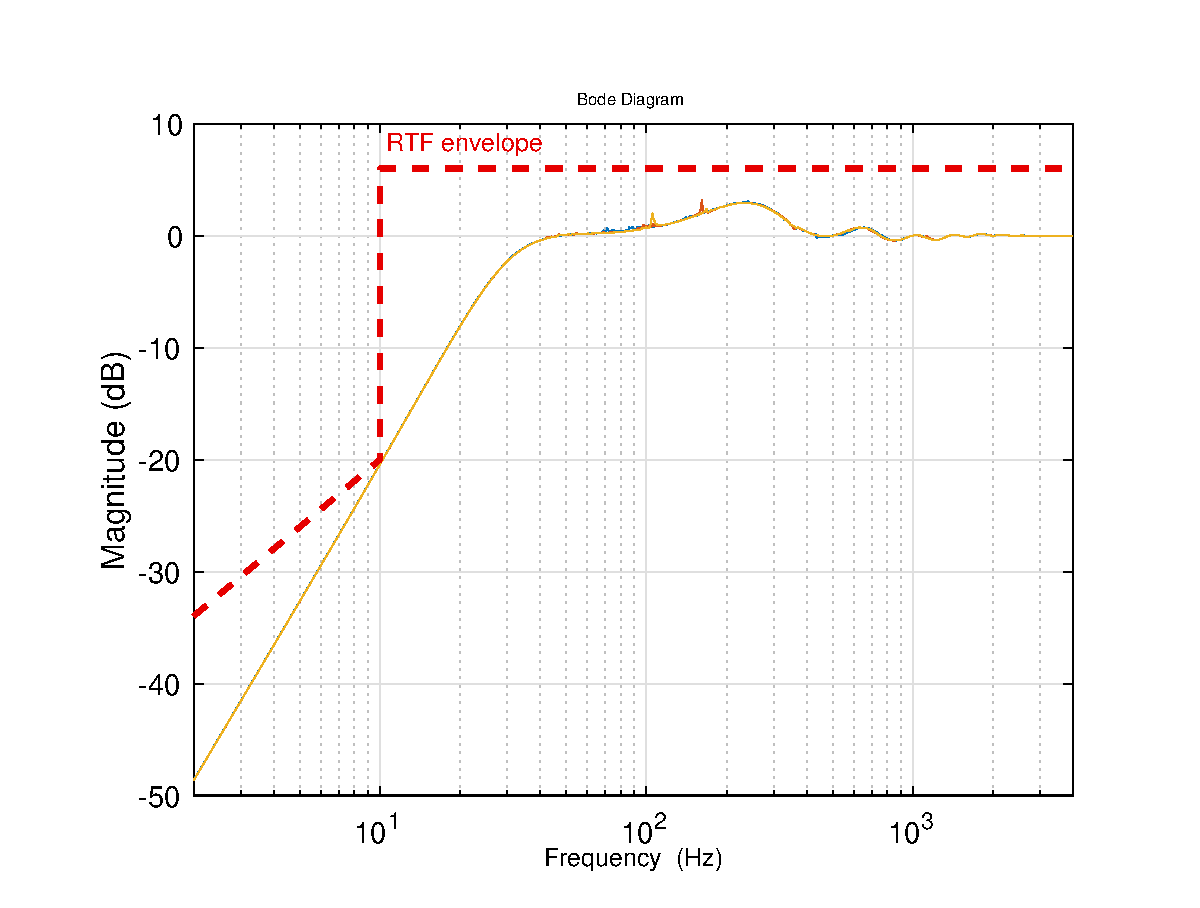
\includegraphics[width=.495\textwidth]{m2s1_ltao_rtf.eps}
  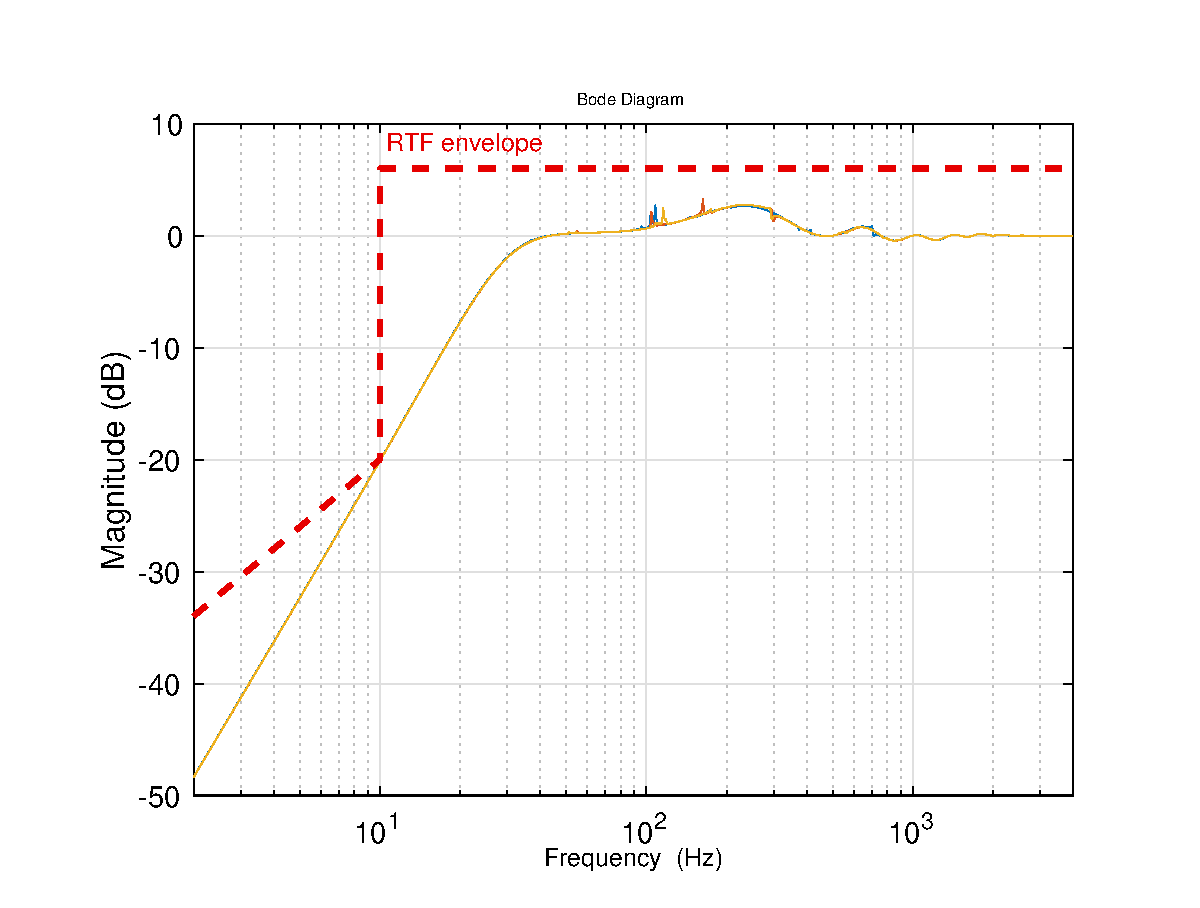
\includegraphics[width=.495\textwidth]{m2s7_ltao_rtf.eps}
  \caption[LTAO sensitivity transfer functions]{LTAO sensitivity transfer functions for segments S1 (left) and S7 (right-hand plot).}
  \label{fig:ltao_rtf_plots}
\end{figure}
The responses are within the requirements. Furthermore, there is almost no difference between the transfer function of segments S1 and S7 (left and right-hand plot, respectively).


\subsection{Control signal transformation matrices}

To map the segment and the global tip-tilt corrections calculated with $C_\text{stt}$ and $C_\text{gtt}$, respectively, into ASM commands, we have used two matrices: $T_\text{ttp2asm} \in \mathbb{R}^{21 \times 21}$ and $T_\text{gtt2sttp} \in \mathbb{R}^{21 \times 2}$. The first transforms segment tip-tilt and piston at the focal plane into ASM commands represented as KL mode coefficients. In the following, the derivation of $T_\text{ttp2asm}$ is approached.

\subsubsection*{Transformation from segment TT to ASM commands}

Denote as $u_\text{asm\_vc}^{(i)}$ the vector of ASM voice-coil forces\footnote{The ASM voice-coil forces are differential forces applied between nodes at the mirror face sheet and the cold plate. The input corresponding to these forces is denoted as \texttt{ASM\_FS-CP\_F} in Figure~\ref{fig:ltaoIM}.} of a particular segment $i \in \{1, \ldots, 7\}$. Using the static solution of the telescope finite-element model (FEM), we obtain the gain matrices $\bar{G}_\text{asm\_fsrb}^{(i)} \in \mathbb{bb}^{675 \times 675}$ and $\bar{G}_\text{asm\_rbm}^{(i)} \in \mathbb{bb}^{6 \times 675}$, such that
\begin{align} \label{eq:static_relations}
    \begin{bmatrix}
        y_\text{fs-rb}^{(i)} \\ y_\text{m2}^{(i)}
    \end{bmatrix} = 
    \begin{bmatrix}
        \bar{G}_\text{asm\_fsrb}^{(i)}
        \\ \bar{G}_\text{asm\_rbm}^{(i)}
    \end{bmatrix} u_\text{asm\_vc}^{(i)}
\end{align}
where $y_\text{fs-rb}^{(i)}$ is the vector of axial displacements between pairs of nodes in the ASM face-sheet (FS) and reference body (RB) and $y_\text{m2}^{(i)}$ is a partition of 
$$y_\text{m2} = \begin{bmatrix}
    y_\text{m2}^{(1) T} & y_\text{m2}^{(2) T} & \cdots & y_\text{m2}^{(7) T}
\end{bmatrix}^T,$$
{\it i.e.}, $y_\text{m2}^{(i)} \in \mathbb{R}^6$ is made up of the M2 rigid-body motions of a the $i^\text{th}$ segment represented in the local coordinate system.

Consider the partitions
\begin{equation}
\label{eq:decomp_lom}
    \begin{bmatrix} 
    L_\text{stt} \\ L_\text{sp} \\ L_\text{gtt}
    \end{bmatrix}
    =
    \begin{bmatrix}
        L_\text{stt\_m1}^{(1)} & \cdots & L_\text{stt\_m1}^{(7)} & L_\text{stt\_m2}^{(1)} & \cdots & L_\text{stt\_m2}^{(7)} \\ L_\text{sp\_m1}^{(1)} & \cdots & L_\text{sp\_m1}^{(7)} & L_\text{sp\_m2}^{(1)} & \cdots & L_\text{sp\_m2}^{(7)} \\ L_\text{gtt\_m1}^{(1)} & \cdots & L_\text{gtt\_m1}^{(7)} & L_\text{gtt\_m2}^{(1)} & \cdots & L_\text{gtt\_m2}^{(7)}
    \end{bmatrix}
\end{equation}
of the LOM matrices presented in \eqref{eq:lom} providing the contributions of each M1 and M2 segment separately. Let
\begin{equation} \label{eq:mo_y}
    y_\text{mo\_fs-rb}^{(i)} = V_\text{KL}^{(i)T} y_\text{fs-rb}^{(i)}
\end{equation}
be the ASM displacement outputs projected onto the KL modal basis and
\begin{equation} \label{eq:mo_u}
    u_\text{asm\_vc}^{(i)} = V_\text{KL}^{(i)} u_\text{mo\_asm}^{(i)}
\end{equation}
the relation between the ASM voice-coil forces and its modal coefficients $u_\text{mo\_asm}^{(i)}$. %
%
That enables us to write
\begin{align}
    y_\text{sttp}^{(i)} &\triangleq \begin{bmatrix}
        L_\text{stt\_m2}^{(i)} \\ L_\text{sp\_m2}^{(i)}
    \end{bmatrix} y_\text{m2}^{(i)} \nonumber \\
    & = \begin{bmatrix}
        L_\text{stt\_m2}^{(i)} \\ L_\text{sp\_m2}^{(i)}
    \end{bmatrix}
    \bar{G}_\text{asm\_rbm}^{(i)}
    u_\text{asm\_vc}^{(i)} \nonumber \\
    \label{eq:asm2ttp}
    & = \begin{bmatrix}
        L_\text{stt\_m2}^{(i)} \\ L_\text{sp\_m2}^{(i)}
    \end{bmatrix}
    \bar{G}_\text{asm\_rbm}^{(i)}
    V_\text{KL}^{(i)} u_\text{mo\_asm}^{(i)}
\end{align}

Thus, from the inverse of the transformation described in \eqref{eq:asm2ttp} and \eqref{eq:static_relations}, it follows that
\begin{equation*}
y_\text{fs-rb}^{(i)}  = 
    \bar{G}_\text{asm\_fsrb}^{(i)}
    V_\text{KL}^{(i)}
    \left(
    \begin{bmatrix}
        L_\text{stt\_m2}^{(i)} \\ L_\text{sp\_m2}^{(i)}
    \end{bmatrix}
    \bar{G}_\text{asm\_rbm}^{(i)}
    V_\text{KL}^{(i)}
    \right)^{-1} y_\text{sttp}^{(i)}
\end{equation*}
and then using \eqref{eq:mo_y} yields to
\begin{equation*}
y_\text{mo\_fs-rb}^{(i)} = V_\text{KL}^{(i)T} 
y_\text{fs-rb}^{(i)}  = 
    \underbrace{
    V_\text{KL}^{(i)T}
    \bar{G}_\text{asm\_fsrb}^{(i)}
    V_\text{KL}^{(i)}
    \left(
    \begin{bmatrix}
        L_\text{stt\_m2}^{(i)} \\ L_\text{sp\_m2}^{(i)}
    \end{bmatrix}
    \bar{G}_\text{asm\_rbm}^{(i)}
    V_\text{KL}^{(i)}
    \right)^{-1}}_{\triangleq T_\text{ttp2asm}^{(i)}}
    y_\text{sttp}^{(i)}.
\end{equation*}

Putting together the transformations of all segments lead to
\begin{equation} \label{eq:ttp2asm}
    T_\text{ttp2asm} = \begin{bmatrix}
    T_\text{ttp2asm}^{(1)} & & \bigcirc  \\
    & \ddots & \\
    \bigcirc  & & T_\text{ttp2asm}^{(7)}
\end{bmatrix}.
\end{equation}

\subsubsection*{Transformation from global TT to ASM commands}

As the mapping from segment tip-tilt and piston (TTP) at the focal plane to the ASM displacements is available, instead of directly obtaining the ASM commands required to compensate global TT modes, as suggested in Figure~\ref{fig:ltao_wfsc_detailed}, we split that task into two steps. First, the transformation $T_\text{gtt2sttp}$ relating global TT and segment TTP is addressed. Then, we use \eqref{eq:ttp2asm} to obtain the ASM compensation commands.

Consider the matrices 
\begin{equation} \label{eq:Cm1m2}
    \Phi_\text{m1m2} = \begin{bmatrix}
    C\left(\texttt{m1\_rbm idxs},\texttt{1:3}\right) \\
    C\left(\texttt{m2\_rbm idxs},\texttt{1:3}\right)
\end{bmatrix}
\in \mathbb{R}^{84 \times 3}
\end{equation}
and
\begin{equation} \label{eq:Cmnt}
    \Phi_\text{AzEl} = \begin{bmatrix}
    \dfrac{1}{n_\text{az\_enc}} \sum\limits_{i=1}^{n_\text{az\_enc}} C\left(\texttt{az\_enc$_i$idx},\texttt{1:3}\right) \\
    \dfrac{1}{n_\text{el\_enc}} 
    \sum\limits_{i=1}^{n_\text{el\_enc}}
    C\left(\texttt{el\_enc$_i$idx},\texttt{1:3}\right)
\end{bmatrix}
\in \mathbb{R}^{2 \times 3}
\end{equation}
built from the first three modes of the output matrix of the telescope structural model represented in the second-order modal state-space form. 
The constants $n_\text{az\_enc}$ and $n_\text{el\_enc}$ denote the number of mount azimuth and elevation encoders, respectively, while \texttt{az\_enc$_i$idx} and \texttt{el\_enc$_i$idx} stand for the indexes of the $i$-th encoder in the output matrix $C$.

Using \eqref{eq:Cm1m2} and \eqref{eq:Cmnt}, one gets 
\begin{equation} \label{eq:mnt2m1m2}
    T_\text{mnt2m12} = \Phi_\text{m1m2} \Phi_\text{AzEl}^\dagger
\end{equation}
mapping mount azimuth and elevation motions into M1 and M2 rigid-body motions and
\begin{equation} \label{eq:gtt2mnt}
    T_\text{gtt2mnt} =  \left(L_\text{gtt} T_\text{mnt2m12}\right)^{-1}
\end{equation}
relating global tip-tilt at the focal plane and the mount axes motion. The symbol ``$\dagger$'' represents the Moore–Penrose inverse.

From \eqref{eq:lom} and \eqref{eq:mnt2m1m2}--\eqref{eq:gtt2mnt}, we get
\begin{align}
   T_\text{gtt2sttp} & = \begin{bmatrix}
    L_\text{stt} \\ L_\text{sp}
\end{bmatrix} T_\text{mnt2m12}T_\text{gtt2mnt} \nonumber \\
\label{eq:gtt2sttp}
    & = \begin{bmatrix}
    L_\text{stt} \\ L_\text{sp}
\end{bmatrix} \Phi_\text{m1m2} \Phi_\text{AzEl}^\dagger \left(  L_\text{gtt}  \Phi_\text{m1m2} \Phi_\text{AzEl}^\dagger \right)^{-1} .
\end{align}
%gtt2sttp = [D_seg_tt; D_seg_piston]*Hk_mnt_m1m2*gtt2mnt


\begin{remark}
    Obtaining the relation between global and segment tip-tilt is not straightforward. To avoid pseudo-inverses of matrices with more rows than columns (leading to undetermined solutions), we exploit the kinematic relations embedded into the telescope structural model represented in the state-space form through matrices $\left(A,B,C\right)$. In summary, the first three structural model eigenmodes reflect the dynamics of all three axes (AZ, EL, and GIR) without flexible forms. Therefore, we can use \eqref{eq:Cm1m2} and \eqref{eq:Cmnt} relating the first three eigenmodes with M1 and M2 rigid-body motions and with the azimuth and elevation axes displacements, respectively, to get the kinematic relation \eqref{eq:mnt2m1m2} between the mount pointing (AZ and EL) and the M1 and M2 rigid-body motions. At last, one combines the optical sensitivity matrices \eqref{eq:lom}, the kinematic relation \eqref{eq:mnt2m1m2}, and the bijective relation \eqref{eq:gtt2mnt} between global tip-tilt and mount pointing (azimuth and elevation) to develop $T_\text{gtt2sttp}$ in \eqref{eq:gtt2sttp}.
\end{remark}



\subsection{Edge sensor control loops}

Figure~\ref{fig:ltao_wfsc_detailed} shows that three blocks comprise the M1 feedforward (FF) control model: the reconstructor of the M1 rigid-body motions, a linear transformation, and a filter.

Denote as $D_{1\text{es}} \in \mathbb{R}^{48 \times 42}$ the interaction matrix relating the M1 rigid-body motions and the $48$-dimensional vector of distances between collimator and retro-reflector edge sensor nodes (Figure~\ref{fig:D1es_sv}). An ideal linear reconstructor is the pseudo-inverse of $D_{1\text{es}}$. However, the edge sensors can not measure the global displacements of the M1 segments, meaning that $D_{1\text{es}}$ is rank deficient, as shown in the right-hand plot of Figure~\ref{fig:D1es_sv} (refer also to \cite{FWN.124} or \cite[Section~4.1]{PistonRej_QPacheco2019}). Among the available strategies to deal with rank deficiency, we have followed one of the strategies proposed in \cite[Section~2.2]{FWN.124}: inverting the truncated singular value decomposition (SVD) of the interaction matrix. So, given the decomposition 
$$D_{1\text{es}} = U_{1\text{es}} \Sigma_{1\text{es}} V_{1\text{es}}^T,$$
and discarding the contribution of the six smallest singular values (corresponding to the global translations and rotations modes), the reconstructor estimating the M1 rigid-body motions from the edge-sensor measurements reads\footnote{For compactness, we have used MatLab notation to represent blocks of matrices. For example, $V_{1\text{es}}(\texttt{1:42,1:36})$ stands for a submatrix with the first 42 rows and the first 36 columns of $V_{1\text{es}}$.} as
\begin{equation} \label{eq:R1es}
    R_{1\text{es}} = V_{1\text{es}}(\texttt{1:42,1:36}) \left(\Sigma_{1\text{es}}(\texttt{1:36,1:36})\right)^{-1} \left(U_{1\text{es}}(\texttt{1:48,1:36})\right)^T.
\end{equation}
%
\begin{figure}[!hbt]
  \centering
  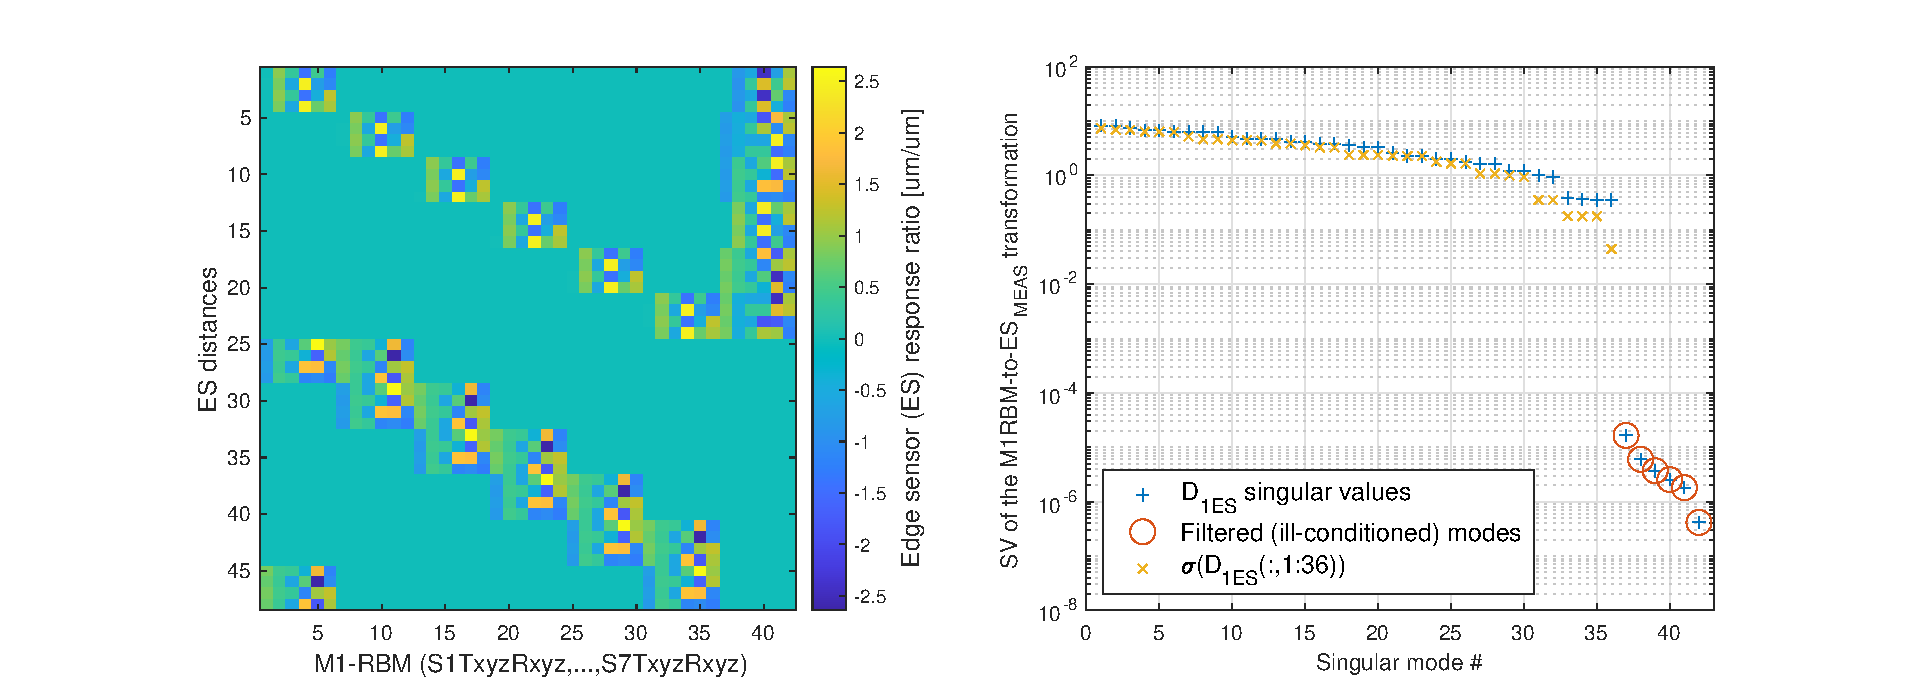
\includegraphics[trim=60 0 60 0, clip, width=\textwidth]{D1es_map_sv.eps}
  \caption[M1 edge sensor interaction matrix]{M1 edge sensor interaction matrix (left) and its singular values (right).}
  \label{fig:D1es_sv}
\end{figure}

From \eqref{eq:decomp_lom} and \eqref{eq:ttp2asm}, the matrix projecting the reconstructed rigid-body motions onto ASM tip-tilt and piston commands is
\begin{equation} \label{eq:Tm1ff}
    T_\text{m1ff} =     T_\text{ttp2asm} \begin{bmatrix}
        L_\text{stt\_m1}^{(1)} & \cdots & L_\text{stt\_m1}^{(7)} \\ L_\text{sp\_m1}^{(1)} & \cdots & L_\text{sp\_m1}^{(7)} 
    \end{bmatrix}.
\end{equation}

The transfer function $F_{1\text{es}}(s)$ represents a second-order Butterworth filter with corner frequency set at \SI{50}{\hertz}. The low-pass filter follows the model used to represent the edge sensor in the M2 subsystem~\cite{ADP_PhasingRep2021}.

The M2 edge sensor control loop is part of AdOptica's design. Here, we assume the same strategy of the M1 feedforward control illustrated in Figure~\ref{fig:ltao_wfsc_detailed}: a linear controller composed of a reconstructor $R_{2\text{es}}$, a linear transformation $T_\text{m2ff}$, and a \SI{50}{\hertz} low-pass Butterworth filter $F_{2\text{es}}$. %
On the left, Figure~\ref{fig:D2es_sv} shows the M2 edge sensor interaction matrix $D_{2\text{es}}$ and its singular values on the right-hand plot.
%
Therefore, analogously to \eqref{eq:R1es}--\eqref{eq:Tm1ff}, it follows that
%
\begin{figure}[!hbt]
  \centering
  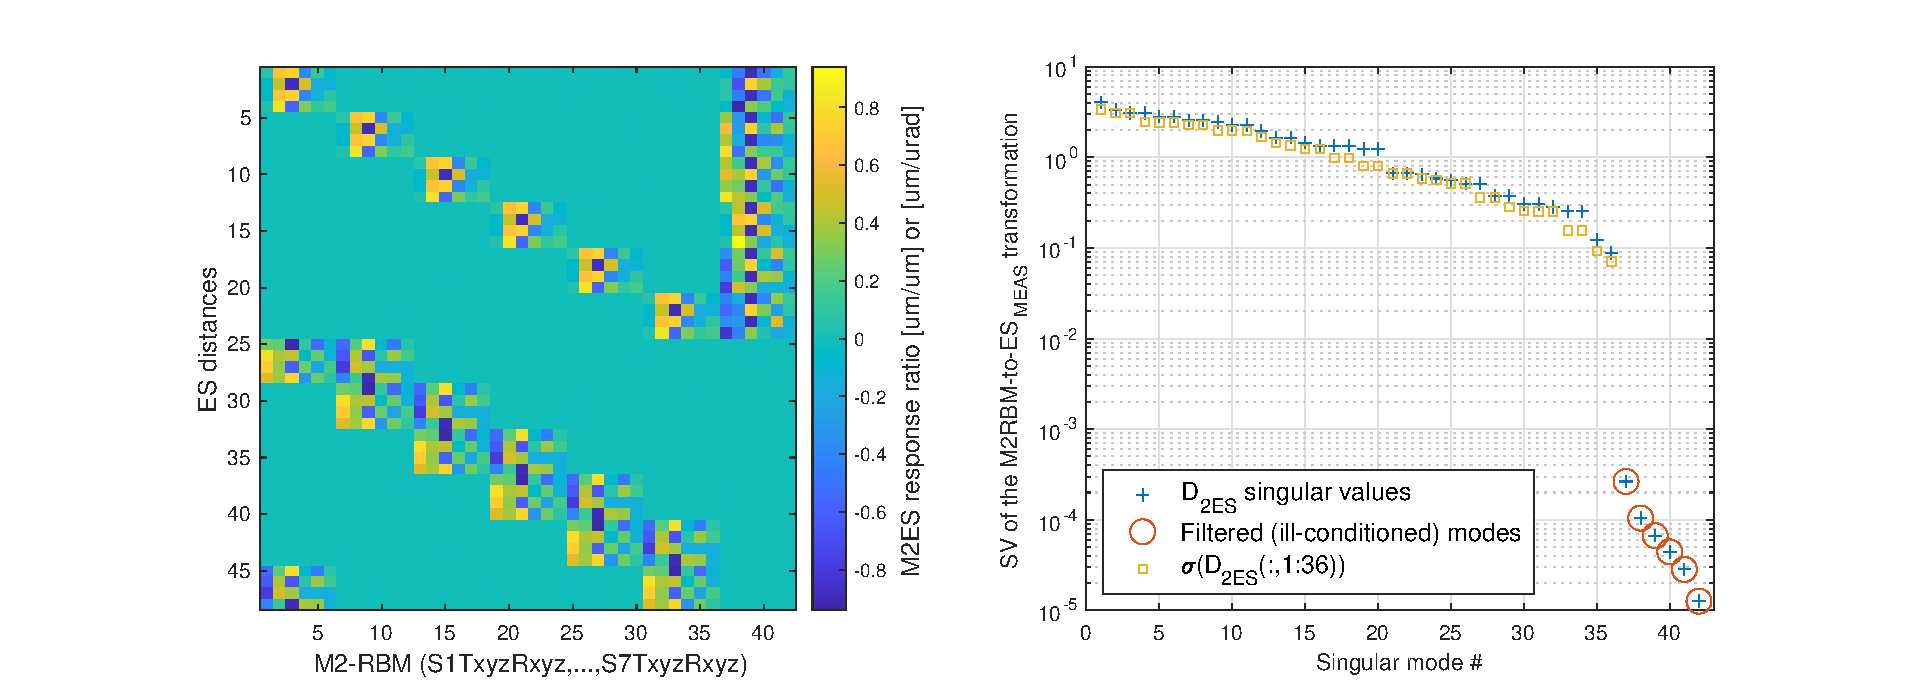
\includegraphics[trim=60 0 60 0, clip, width=\textwidth]{D2es_map_sv.eps}
  \caption{M2 edge sensor interaction matrix.}
  \label{fig:D2es_sv}
\end{figure}
%
\begin{equation*}
  R_{2\text{es}} = V_{2\text{es}}(\texttt{1:42,1:36}) \left(\Sigma_{2\text{es}}(\texttt{1:36,1:36})\right)^{-1} \left(U_{2\text{es}}(\texttt{1:48,1:36})\right)^T,
\end{equation*}
where $D_{2\text{es}} = U_{2\text{es}} \Sigma_{2\text{es}} V_{2\text{es}}^T$ is the matrix mapping the rigid motions of the M2 reference bodies into the $48$-dimensional vector of the edge sensor distance measurements, and
\begin{equation*}
  T_\text{m2ff} =     T_\text{ttp2asm} \begin{bmatrix}
    L_\text{stt\_m2}^{(1)} & \cdots & L_\text{stt\_m2}^{(7)} \\ L_\text{sp\_m2}^{(1)} & \cdots & L_\text{sp\_m2}^{(7)} 
\end{bmatrix}.
\end{equation*}



%\section{Concluding Remarks}

\printbibliography

\appendix

\newpage

\section{M2 Control System Model}
\label{sec:m2_control}

\subsection{ASM inner loop control}
\label{sec:asm-ctrl}

Figure~\ref{fig:modal_asm_loop} illustrates the ASM inner loop controller model. An input shaping filter block, a feedback compensator, and a feedforward term compose the ASM inner loop controller of each segment.  %
%
\begin{figure}[!hbt]
  \centering
  \includegraphics[width=0.95\textwidth]{asm_controller.pdf}
  \caption{ASM inner loop controller block diagram.}
  \label{fig:modal_asm_loop}
\end{figure}

Using a $4^{th}$--order Bessel filter with corner frequency $\omega_{\beta f}=2 \pi 2.2 \times 10^3$\si{rad/s} the command pre--shape
\begin{equation}
  \label{eq:4thBessel}
  F_\text{pre}(s) = 
    \frac{\beta_0 \omega_{\beta f}^4}{\beta_4 \omega_{\beta f}^0 s^4 + \beta_3 \omega_{\beta f}^1 s^3 + \beta_2 \omega_{\beta f}^2 s^2 + \beta_1 \omega_{\beta f}^3 s + \beta_0 \omega_{\beta f}^4}    
\end{equation}
aims at smoothing the $n_m$--dimensional modal command vector $R_\text{mo\_asm}(s)$. Table~\ref*{tab:bessel_f_prototype} provides the filter prototype coefficients $\beta_l$, for $l=\{0,1,\dots,4\}$.
%
\begin{table}[!htb]
  \centering
  \caption{$4^{th}$--order Bessel filter prototype coefficients.}
  \label{tab:bessel_f_prototype}
  \begin{tabular}{|c|c|c|c|c|}
  \hline
  $\beta_4$ & $\beta_3$ & $\beta_2$ & $\beta_1$ & $\beta_0$ \\
  \hline
  1.0 & 3.12393994 & 4.39155033 & 3.20108587 & 1.0\\
  \hline
  \end{tabular}
\end{table}


A proportional--integral compensator 
\begin{equation*}
%\label{eq:pi_CT}
C_\text{PI}(s) = I_{n_m} \left(k_p + \frac{k_i}{s} \right)
\end{equation*}
and derivative action proportional to $k_d$ compose the feedback controller 
\[C_\text{FB}(s) = -C_\text{PI}(s) + k_d H_\text{pd}(s) \]
where the transfer function
\begin{equation*}
  H_\text{pd}(s) = I_{n_m} \frac{s}{2\pi f_{c\text{pd}}s + 1} , 
  \end{equation*}
performs a filtered differentiation with $f_{c\text{pd}} = \SI{4}{kHz}$. %
The feedback signal is the vector of relative displacements between the face sheet (FS) and the reference body (RB) nodes $y_\text{fs-rb}$ projected onto the orthonormal base $V_\text{KL}^{(i)T}$, the same signal used to model the fluid damping forces (see Figure~\ref{fig:ltaoIM}).

%
%The feedforward (FF) control has a static and dynamic contribution. The purpose of the static contribution is to provide (in advance) the static forces required to apply a particular command, statically decoupling all the commanded degrees of freedom. The dynamic FF term aims at pre--compensating (in open--loop) the system dynamics during the command transients. %
%
For each ASM segment, the Laplace transform of the feedforward compensation is 
\begin{equation}
\label{eq:U_FF_static_dyn}
U_\text{FF}(s) = \underbrace{K_s F_\text{pre}(s) R_\text{mo\_asm}(s)}_{\text{static}} + 
\underbrace{ \left(
k_b H_{f1\text{d}}(s) + k_m H_{f2\text{d}}(s) \right) R_\text{mo\_asm}(s)}_{\text{dynamic}},
\end{equation}
where $K_s \in \mathbb{R}^{n_m \times n_m}$ is the modal stiffness matrix $\Psi_V$, $I_{n_m}$ denotes the identity matrix of dimension $n_m$, and
\begin{align*}
  H_{f1\text{d}}(s) & =  s I_{n_m} F_\text{pre}(s) \\
  H_{f2\text{d}}(s) & = s^2 I_{n_m} F_\text{pre}(s)
  .
  \end{align*}
The mass $k_b$ and the damping $k_m$ factors are scalar gains.

Consider the $n_a \times n_a$ matrix relating the relative nodal displacements (\texttt{ASM\_FS-RB\_delta\_D} output) due to relative nodal forces (\texttt{ASM\_FS-CP\_delta\_F} input), denoted as $\bar{G}_\text{asm\_fsrb}$ in \eqref{eq:static_relations}. The modal ASM stiffness matrix for a particular segment $i \in \{1,2,\ldots,7\}$ is
\begin{equation}
\label{eq:Psi_V}
\Psi_V = \left( V_\text{KL}^{(i)T} \bar{G}_\text{asm\_fsrb} V_\text{KL}^{(i)} \right)^{-1}.
\end{equation}


One can exploit linear system realization theory to obtain the transfer functions $s F_\text{pre}(s)$ and $s^2 F_\text{pre}(s)$ in \eqref{eq:U_FF_static_dyn} without explicitly performing time--derivative operations. Consider the tuple $\left( A_f, B_f, C_f \right)$ representing the $4^{th}$--order Bessel filter transfer function \eqref{eq:4thBessel} in the state--space form, such that
\begin{equation}
\label{eq:Fpre}
F_\text{pre}(s) = C_f\left(s I_4-A_f\right)^{-1}B_f.
\end{equation}
%
It follows that the (filtered) ASM velocity and acceleration command transfer functions can be written as
\begin{align}
s F_\text{pre}(s) & = \left(C_f A_f\right)\left(s I_4-A_f\right)^{-1} B_f \label{eq:Fpre_dot} \\
s^2 F_\text{pre}(s) & = \left(C_f A_f^2\right)\left(s I_4-A_f\right)^{-1} B_f . \label{eq:Fpre_ddot}
\end{align}

Table~\ref{tab:ASM_inner_ctrl_par} summarizes the ASM controller model parameter values. Figure~\ref{fig:asm_modal_resp} shows the ASM open- (left) and closed-loop (right) responses of segment S7 for the first three KL modes. On the right-hand plot, we also indicate the \SI{800}{\hertz} bandwidth requirement \cite[REQ-L3-OAD-35459]{OAD}. Those modal frequency responses \cite{GMT.DOC.05941} were calculated using the structural model \texttt{20230131\_1605\_zen\_30$\ldots$\_202111} and considering $0.5$\% structural damping.
\begin{table}[!htb]
\centering
\caption[ASM inner loop controller model parameters]{ASM inner loop controller model parameters~\cite{ADP_PhasingRep2021}.}
\label{tab:ASM_inner_ctrl_par}
\begin{tabular}{|c|c|c|c|c|c|}
\hline
$k_p$ \SI{}{(N/m)} & $k_i$ \SI{}{(N/m s)} & $k_d$ \SI{}{(Ns/m)} & $k_m$ \SI{}{(Ns\textsuperscript{2}/m)} & $k_b$ \SI{}{(Ns/m)} & $K_s$ \SI{}{(N/m)} \\
\hline
$7 \times 10^4$ & $5 \times 10^5$ & $24.5$ & $1.12 \times 10^{-2}$ & $33.6$ & $\Psi_V$ (see~\eqref{eq:Psi_V})\\
\hline
\end{tabular}
\end{table}
\begin{figure}[!hbt]
  \centering
  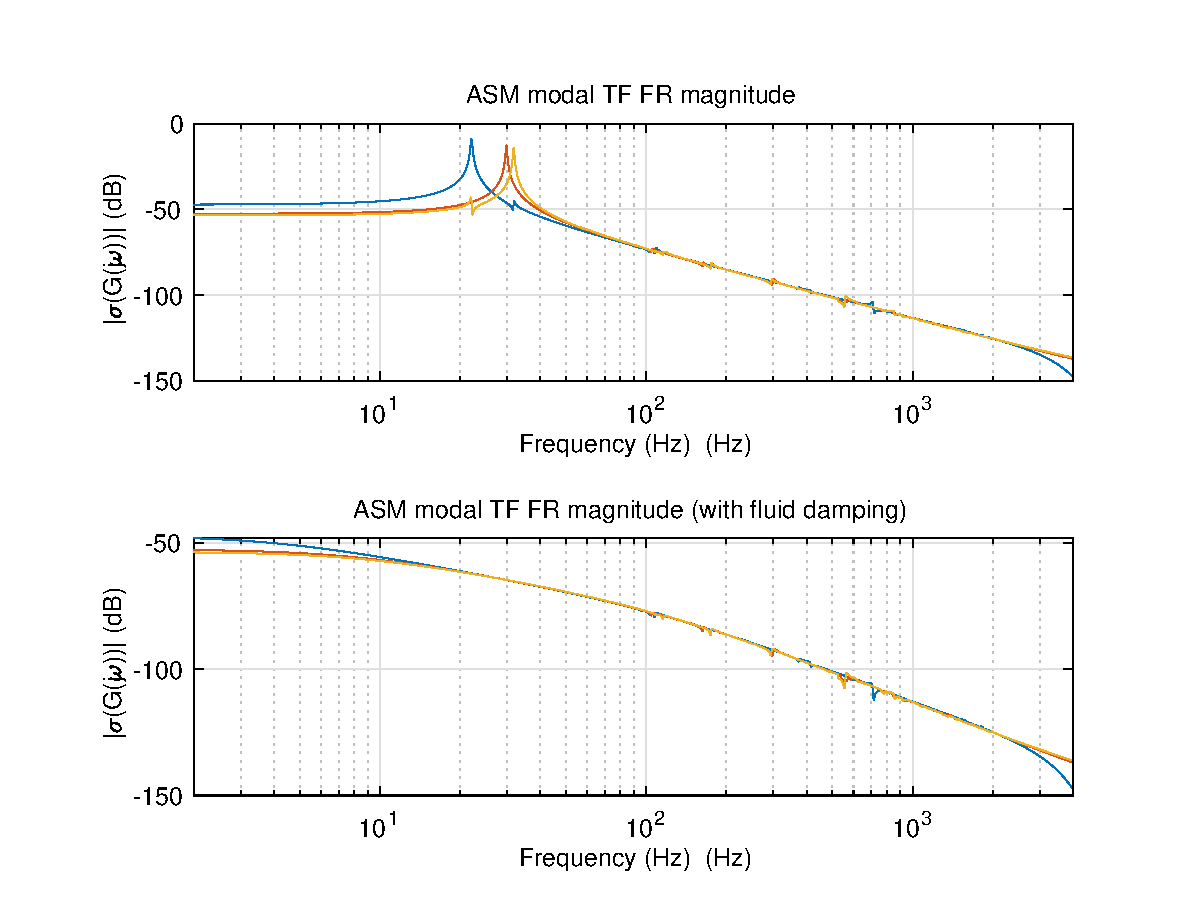
\includegraphics[width=.495\textwidth]{m2s7_asm_ol.eps}
  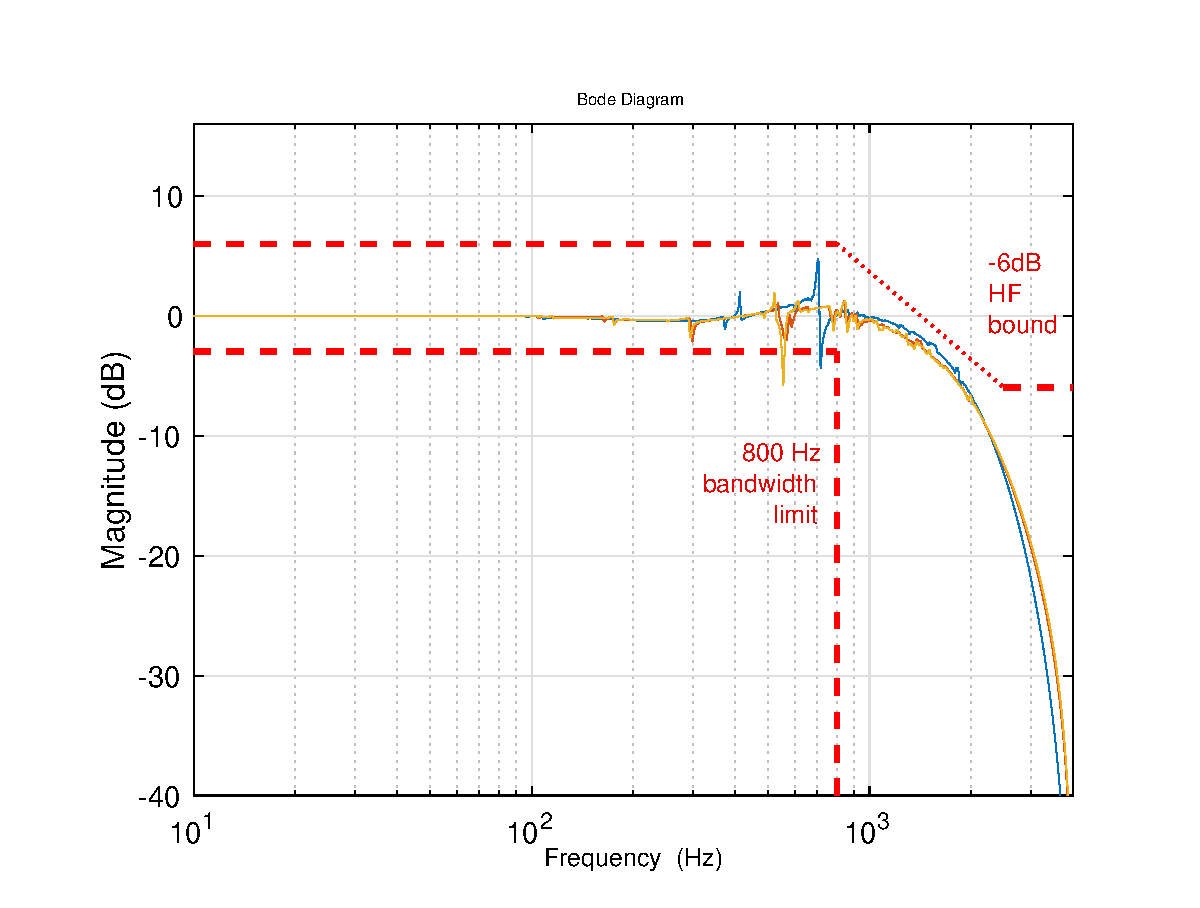
\includegraphics[width=.495\textwidth]{m2s7_asm_cl.eps}
  \caption[ASM segment S7 modal responses.]{Adaptive secondary mirror open- and closed-loop responses.}
  \label{fig:asm_modal_resp}
\end{figure}

\subsection{M2 positioner}
\label{sec:m2p-ctrl}

The Observatory Requirement Document (OAD)~\cite{OAD} stipulates through REQ--L3--OAD--35039 that the M2 positioner (M2P) shall provide a bandwidth of \SI{2}{Hz} while tracks the rigid--body motion commands.

The M2P controller computes the differential forces (\textsf{M2P\_F}), which lengthen or shorten the positioner actuators. Their lengths are the control loop feedback signals. The lengths of the M2P actuators are obtained from differential displacements of the nodes located at the extremes of the rod representing each actuator \textsf{M2P\_D}. The frequency response magnitude of the transfer functions from \textsf{M2P\_F} to \textsf{M2P\_D}, denoted hereafter as $G_\text{m2p}(s)$, are shown in Figure~\ref{fig:M2P_G}. %
%
\begin{figure}[!hbt]
    \vspace{6pt}
    \centering
    \includegraphics[width=\textwidth]{/Users/rromano/Workspace/reports_slides/asm_im-doc/ctrl_sec_images/M2P_G.eps}
    \caption{Frequency response magnitude of the M2 positioner actuators.}
    \label{fig:M2P_G}
\end{figure}
%
At the frequency range relevant for the specified closed--loop bandwidth, the model behaves like a static gain equal to the reciprocal of the stiffness of the M2P actuators, which is $k_\text{m2p}=\SI{158}{N/um}$. %\footnote{...}\todo{Explain difference w.r.t. FEA.}.
To provide enough gain at low frequencies and attenuate the modes above \SI{20}{Hz}, we use an M2P feedback controller with an integral term and a low--pass filter with a corner frequency at \SI{10}{Hz}, i.e.,
\begin{equation}
\label{eq:C_m2p}
C_\text{m2p}(s) = I_{42} \frac{k_{i\text{m2p}}}{s} \frac{1}{\frac{1}{\left(2\pi10\right)^2}s^2 + \frac{1}{2\pi10}s+1} ,
\end{equation}
where $I_{42}$ is a 42--dimensional identity matrix and the assumed integral gain $k_{i\text{m2p}} = 2 \pi 2 k_\text{m2p}$ leads to a unitary magnitude crossover frequency of \SI{2}{Hz}, i.e., 
\[\left|G_\text{m2p}(j\omega_0)C_\text{m2p}(j\omega_0)\right|_{\omega_0 = 2\pi2} = I_{42} .\]
%where $G_\text{m2p}(s)$ is the matrix transfer function relating the M2 differential forces \textsf{M2P\_F} and the differential displacement outputs \textsf{M2P\_D}.

The Nichols chart on the right side of Figure~\ref{fig:m2P_nichols_T} shows quite comfortable margins as the loop frequency response is distant to the dashed red line, which indicates the robustness boundary assuming a $0.5$ vector margin\footnote{The vector margin (VM) is the reciprocal of the maximum value of the loop sensitivity transfer function $S\left(j\omega\right)$ magnitude, i.e.$$\text{VM}=\frac{1}{\max \left|S(j\omega)\right|}.$$} (VM). %
%
\begin{figure}[!hbt]
    \vspace{6pt}
    \centering
    \includegraphics[width=\textwidth]{/Users/rromano/Workspace/reports_slides/asm_im-doc/ctrl_sec_images/m2P_nichols_T.eps}
    \caption{M2 positioner control loop characterization plots.}
    \label{fig:m2P_nichols_T}
\end{figure}
%
On the right side, one can see the closed--loop (complementary sensitivity) response of all the M2 positioner actuators. The control loop achieves the required bandwidth of \SI{2}{Hz} using the proposed feedback controller. %; see~\eqref{eq:C_m2p}.

% The matrix $K_\text{m2pT}$ maps the M2 rigid--body motion commands into reference lengths for the positioner actuators. Though $K_\text{m2pT}$ can be obtained analytically from the M2P geometry, in the context of Integrated modeling, we have computed it using the telescope structural dynamics model represented in the state--space form through the tuple $(A, B, C)$. Let $B_\textsf{M2P\_F}$ denote the partition of $B$ composed of the columns corresponding to the M2P differential force inputs \textsf{M2P\_F}. 
% Also, define $C_\textsf{M2P\_D}$ and $C_\textsf{M2\_RBM}$ as matrices constructed from the rows of $C$ corresponding to the M2P differential displacements  \textsf{M2P\_D} and the M2 rigid--body motions (\textsf{M2\_RBM}), respectively. Then
% \begin{equation*}
% K_\text{m2pT} = \bar{G}_1 \bar{G}_2^{-1},
% \end{equation*}
% where
% \begin{align*}
% \bar{G}_1 & = - C_\textsf{M2P\_D} A^{-1} B_\textsf{M2P\_F} \\
% \bar{G}_2 & = - C_\textsf{M2\_RBM} A^{-1} B_\textsf{M2P\_F}.
% \end{align*}
% %Coming from $D$, the direct feedthrough submatrices $D_1$ and $D_2$ relate the \textsf{M2P\_F} inputs and the outputs \textsf{M2P\_D} and \textsf{M2\_RBM}, respectively.


\end{document}
